\section{Auswertung} \label{sec:auswertung}

Im Folgenden sollen auf Basis der aufgenommenen Messwerte
die Halbwertszeiten von aktiviertem Vanadium und Rhodium bestimmt werden.
Die nachstehenden Messwerte wurden nicht bearbeitet
und beinhalten daher insbesondere die Untergrundrate.
Diese wurde in \autoref{sec:auswertung:untergrundrate} bestimmt
und anschließend ohne weitere Erwähnung von den Messwerten subtrahiert.

\begin{table}[H]
  \centering
  \caption{Übersicht der für Vanadium aufgenommenen Messwerte \cite{datenundhinweise}.}
  \label{tab:messwerte_vanadium}
  \begin{tabular}{c c | c c}
  \toprule
  $t [\si{\second}]$ &
  $N [\si{{Imp} \per 30 \second}]$ &
  $t [\si{\second}]$ &
  $N [\si{{Imp} \per 30 \second}]$ \\
  \midrule
  \num{30}   & \num{189} ± \num{13.7} & \num{690}  & \num{35} ± \num{5.9}   \\
\num{60}   & \num{197} ± \num{14.0} & \num{720}  & \num{19} ± \num{4.4}   \\
\num{90}   & \num{150} ± \num{12.2} & \num{750}  & \num{28} ± \num{5.3}   \\
\num{120}  & \num{159} ± \num{12.6} & \num{780}  & \num{27} ± \num{5.2}   \\
\num{150}  & \num{155} ± \num{12.4} & \num{810}  & \num{36} ± \num{6.0}   \\
\num{180}  & \num{132} ± \num{11.5} & \num{840}  & \num{25} ± \num{5.0}   \\
\num{210}  & \num{117} ± \num{10.8} & \num{870}  & \num{29} ± \num{5.4}   \\
\num{240}  & \num{107} ± \num{10.3} & \num{900}  & \num{18} ± \num{4.2}   \\
\num{270}  & \num{94} ± \num{9.7}   & \num{930}  & \num{17} ± \num{4.1}   \\
\num{300}  & \num{100} ± \num{10.0} & \num{960}  & \num{24} ± \num{4.9}   \\
\num{330}  & \num{79} ± \num{8.9}   & \num{990}  & \num{21} ± \num{4.6}   \\
\num{360}  & \num{69} ± \num{8.3}   & \num{1020} & \num{25} ± \num{5.0}   \\
\num{390}  & \num{81} ± \num{9.0}   & \num{1050} & \num{21} ± \num{4.6}   \\
\num{420}  & \num{46} ± \num{6.8}   & \num{1080} & \num{24} ± \num{4.9}   \\
\num{450}  & \num{49} ± \num{7.0}   & \num{1110} & \num{25} ± \num{5.0}   \\
\num{480}  & \num{61} ± \num{7.8}   & \num{1140} & \num{17} ± \num{4.1}   \\
\num{510}  & \num{56} ± \num{7.5}   & \num{1170} & \num{20} ± \num{4.5}   \\
\num{540}  & \num{40} ± \num{6.3}   & \num{1200} & \num{19} ± \num{4.4}   \\
\num{570}  & \num{45} ± \num{6.7}   & \num{1230} & \num{20} ± \num{4.5}   \\
\num{600}  & \num{32} ± \num{5.7}   & \num{1260} & \num{18} ± \num{4.2}   \\
\num{630}  & \num{27} ± \num{5.2}   & \num{1290} & \num{16} ± \num{4.0}   \\
\num{660}  & \num{43} ± \num{6.6}   & \num{1320} & \num{17} ± \num{4.1}   \\

  \bottomrule
  \end{tabular}
\end{table}

\begin{table}[H]
  \centering
  \caption{Übersicht der für Rhodium aufgenommenen Messwerte \cite{datenundhinweise}.}
  \label{tab:messwerte_rhodium}
  \begin{tabular}{c c | c c}
  \toprule
  $t [\si{\second}]$ &
  $N [\si{{Imp} \per 15 \second}]$ &
  $t [\si{\second}]$ &
  $N [\si{{Imp} \per 15 \second}]$ \\
  \midrule
  \num{15}  & \num{667} ± \num{25.8} & \num{345} & \num{36} ± \num{6.0}   \\
\num{30}  & \num{585} ± \num{24.2} & \num{360} & \num{38} ± \num{6.2}   \\
\num{45}  & \num{474} ± \num{21.8} & \num{375} & \num{34} ± \num{5.8}   \\
\num{60}  & \num{399} ± \num{20.0} & \num{390} & \num{40} ± \num{6.3}   \\
\num{75}  & \num{304} ± \num{17.4} & \num{405} & \num{21} ± \num{4.6}   \\
\num{90}  & \num{253} ± \num{15.9} & \num{420} & \num{35} ± \num{5.9}   \\
\num{105} & \num{213} ± \num{14.6} & \num{435} & \num{33} ± \num{5.7}   \\
\num{120} & \num{173} ± \num{13.2} & \num{450} & \num{36} ± \num{6.0}   \\
\num{135} & \num{152} ± \num{12.3} & \num{465} & \num{20} ± \num{4.5}   \\
\num{150} & \num{126} ± \num{11.2} & \num{480} & \num{24} ± \num{4.9}   \\
\num{165} & \num{111} ± \num{10.5} & \num{495} & \num{30} ± \num{5.5}   \\
\num{180} & \num{92} ± \num{9.6}   & \num{510} & \num{30} ± \num{5.5}   \\
\num{195} & \num{79} ± \num{8.9}   & \num{525} & \num{26} ± \num{5.1}   \\
\num{210} & \num{74} ± \num{8.6}   & \num{540} & \num{28} ± \num{5.3}   \\
\num{225} & \num{60} ± \num{7.7}   & \num{555} & \num{23} ± \num{4.8}   \\
\num{240} & \num{52} ± \num{7.2}   & \num{570} & \num{20} ± \num{4.5}   \\
\num{255} & \num{56} ± \num{7.5}   & \num{585} & \num{28} ± \num{5.3}   \\
\num{270} & \num{53} ± \num{7.3}   & \num{600} & \num{17} ± \num{4.1}   \\
\num{285} & \num{41} ± \num{6.4}   & \num{615} & \num{26} ± \num{5.1}   \\
\num{300} & \num{36} ± \num{6.0}   & \num{630} & \num{19} ± \num{4.4}   \\
\num{315} & \num{37} ± \num{6.1}   & \num{645} & \num{13} ± \num{3.6}   \\
\num{330} & \num{32} ± \num{5.7}   & \num{660} & \num{17} ± \num{4.1}   \\

  \bottomrule
  \end{tabular}
\end{table}

\subsection{Bestimmung der Untergrundrate}
\label{sec:auswertung:untergrundrate}
Zur Bestimmung der Untergrundrate $N_U$ wurden mehrere Messungen
über ein Messintervall $t = \SI{300}{\second}$ durchgeführt:

\begin{align*}
  N_U &= \{129, 143, 144, 136, 139, 126, 158\} \\
  \overline{N_U} &= \SI{139 \pm 4}{\per{300}\second} = \SI{0.464 \pm 0.013}{\per\second} \\
\end{align*}

\subsection{Bestimmung der Halbwertszeit von Vanadium}
\label{sec:auswertung:vanadium}
In \autoref{fig:plot1_log} sind die Messwerte und zwei Fit-Funktionen dargestellt,
auf die im Folgenden näher eingegangen wird.
Die grau gestrichelten Linien markieren die Halbwertszeit und die doppelte Halbwertszeit,
die aus dem ersten Fit ermittelt wurden.

Hier wurde der Fit durch Anpassung des \hyperref[eqn:zerfallsgesetz]{Zerfallsgesetzes} bestimmt,
unter Zuhilfenahme von \textit{scipy}.

Die folgenden Parameter wurden berechnet:
\begin{align*}
  N_\text{0, fit} &= \SI{6.964 \pm 0.185}{\per\second} \\
  λ_\text{fit} &= \SI{0.00342 \pm 0.00012}{\per\second} \\
\end{align*}
Daraus ergibt sich eine (ungefähre) Halbwertszeit von
\[ T_\text{½} = \SI{203 \pm 7}{\second} \; . \]

Unter Verwendung dieser wurde ein zweiter Fit berechnet,
der nur auf den Messwerten bis zur doppelten (ungefähren) Halbwertszeit beruht,
um die aus dem Übergang in den Untergrund resultierende Ungenauigkeit auszulassen.

\begin{align*}
  N_\text{0, fit} &= \SI{7.289 \pm 0.530}{\per\second} \\
  λ_\text{fit} &= \SI{0.00358 \pm 0.0002}{\per\second} \\
\end{align*}
Die genauere Halbwertszeit beträgt somit
\[ T_\text{½, fit} = \SI{194 \pm 11}{\second} \; . \]

\begin{figure}
  \centering
  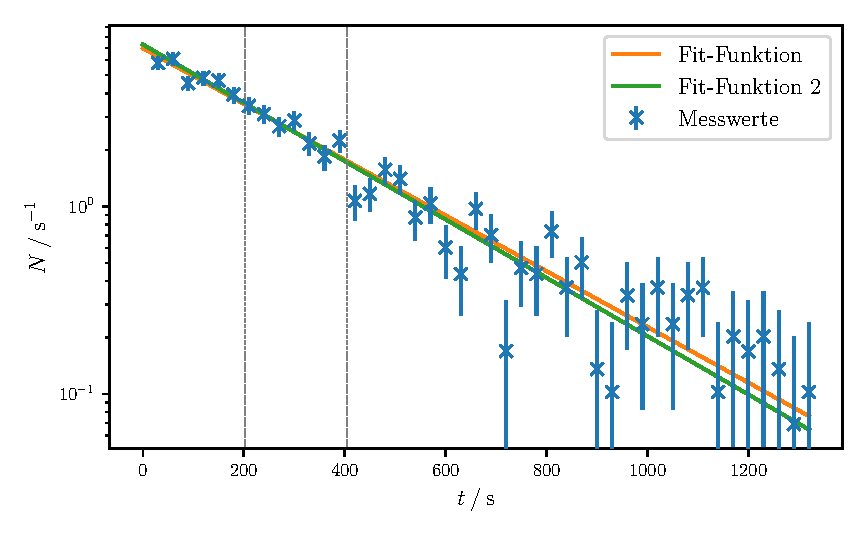
\includegraphics[width=\textwidth]{build/plot1_log.pdf}
  \caption{Halblogarithmische Darstellung der berechneten Zählraten und Fits zu Vanadium.}
  \label{fig:plot1_log}
\end{figure}

\begin{figure}
  \centering
  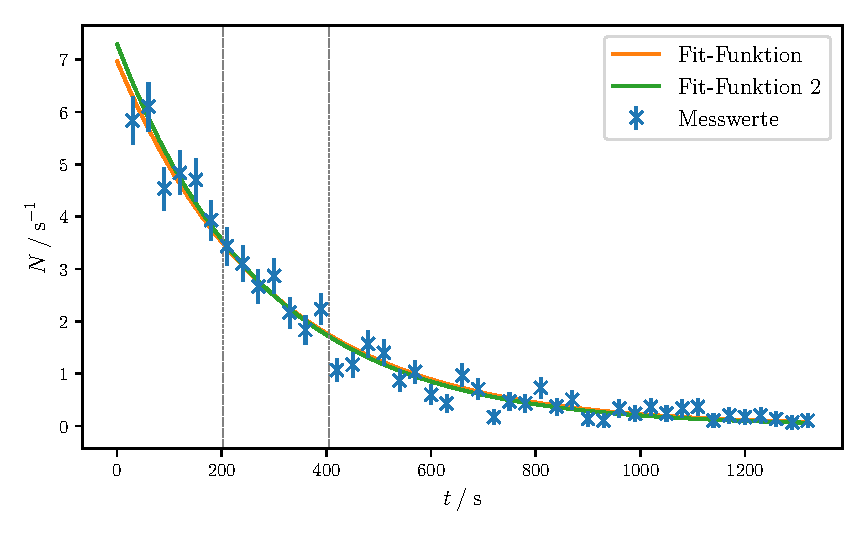
\includegraphics[width=0.75\textwidth]{build/plot1_lin.pdf}
  \caption{Lineare Darstellung der berechneten Zählraten und Fits zu Vanadium.}
  \label{fig:plot1_lin}
\end{figure}


\subsection{Bestimmung der Halbwertszeit von Rhodium}
Die Bestimmung der Halbwertszeit von Rhodium gliedert sich in mehrere Schritte auf,
da Rhodium zwei unterschiedlich schnelle Zerfallskanäle besitzt (siehe \autoref{sec:theorie:zerfall_instabiler_isotope}).
In \autoref{fig:plot2_log} ist daher ein \enquote{Knick} in den Messwerten erkennbar
(gestrichelte Linie bei $\SI{240}{\second}$),
nach welchem nur noch der langlebige Zerfall einen signifikanten Beitrag zur Zählrate leistet.

Zunächst sei hier eine kurze Herleitung der benutzten Regression angegeben:
\begin{align*}
  N(t) &= N_0 e^{-\lambda t}
  \tag{\hyperref[eqn:zerfallsgesetz]{Zerfallsgesetz}} \\
  \ln \left( \frac{N(t)}{N_0} \right) &= - \lambda t \\
  \ln{N(t)} &= \underbrace{(- \lambda)}_\text{Steigung} t + \underbrace{\ln{N_0}}_\text{Achsenabschnitt} \\
\end{align*}
Die Halbwertszeit berechnet sich dann gemäß \autoref{eqn:Halbwertszeit}.

\subsubsection{langsamer Zerfall}
\label{sec:auswertung:rhodium:langsam}
Um die Zerfallskonstante $\lambda_\text{langsam}$ für den langsamen Zerfall zu bestimmen,
wurde $\ln{N(t)}$ gegen die Zeit $t$ aufgetragen
und eine Regressiongerade (orangene Gerade in \autoref{fig:plot2_log})
für die Zeit nach $\SI{240}{\second}$ berechnet.
Die Parameter der Regressiongerade
$\ln{N_\text{langsam}} = mt+n$
sind
\begin{align*}
  m &= -0.00327 \pm 0.0004 \\
  n &= 1.839 \\
\end{align*}
und somit
\begin{align*}
  λ_\text{langsam} &= \SI{0.00327 \pm 0.0004}{\per\second} \\
  T_\text{½, langsam} &= \SI{212 \pm 26}{\second} \; . \\
\end{align*}

\subsubsection{schneller Zerfall}
\label{sec:auswertung:rhodium:schnell}
Um die Zerfallskonstante des schnelleren Zerfalls zu bestimmen,
wird die zugehörige Zählrate isoliert,
indem aus der Fortsetzung der Fit-Funktion $\ln{N_\text{langsam}}$ (orange)
die Zählrate $N_\text{langsam}$ durch Exponentiation ermittelt
und diese von der gemessenen Zählrate subtrahiert wird,
woraufhin erneut der Logarithmus angewandt wird.
Das Ergebnis ist $\ln{N_\text{schnell}}$ (rot).
% Es wurde auch $\ln{N_\text{schnell} + N_\text{langsam}}$ dargestellt (lila).

Auch hierfür wurde eine Regressionsrechnung durchgeführt.
% Wieder wurde eine Regressionsrechnung durchgeführt.
Dabei ergaben sich die Parameter
\begin{align*}
  m &= -0.0190 \pm 0.0007 \\
  n &= 4.137 \\
\end{align*}
und somit
\begin{align*}
  λ_\text{schnell} &= \SI{0.0190 \pm 0.0007}{\per\second} \\
  T_\text{½, schnell} &= \SI{36.5 \pm 1.4}{\second} \; . \\
\end{align*}

\begin{figure}
  \centering
  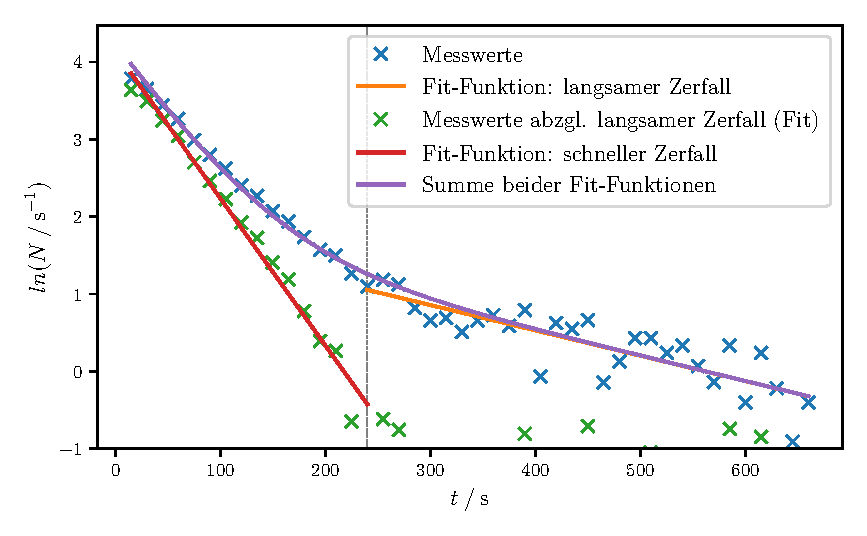
\includegraphics[width=\textwidth]{build/plot2_log.pdf}
  \caption{Halblogarithmische Darstellung der berechneten Zählraten und Fits zu Rhodium.}
  \label{fig:plot2_log}
\end{figure}

\begin{figure}
  \centering
  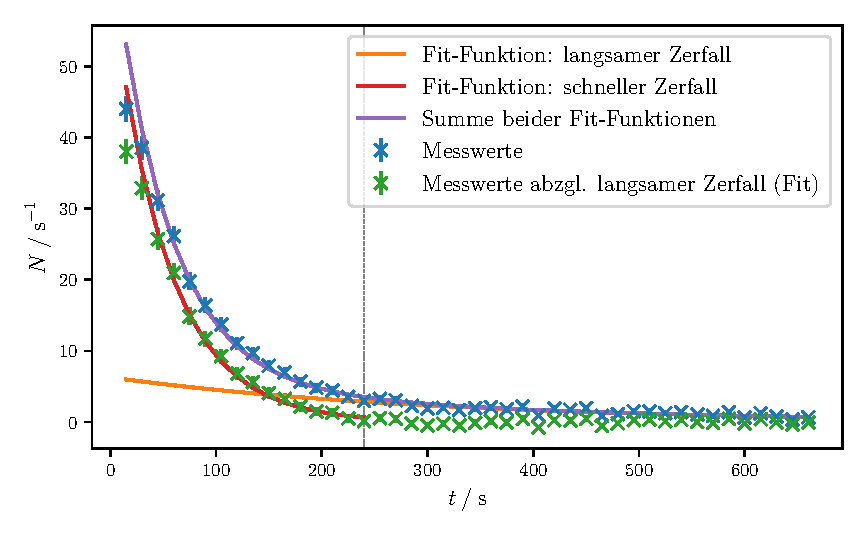
\includegraphics[width=0.75\textwidth]{build/plot2_lin.pdf}
  \caption{Lineare Darstellung der berechneten Zählraten und Fits zu Rhodium.}
  \label{fig:plot2_lin}
\end{figure}
